
\setcounter{section}{0}
\textbf{Chuyển động ném ngang}
\begin{center}
	\begin{tabular}{|m{8cm}|m{8cm}|}
		\hline
		Chuyển động thành phần theo trục O$x$ là chuyển động thẳng đều	& Chuyển động thành phần theo trục O$y$ là chuyển động rơi tự do  \\
		\hline
		\begin{equation*}
			a_{\text{x}}=0.
		\end{equation*} & 
		\begin{equation*}
			a_{\text{y}}=g.
		\end{equation*}  \\
		\hline
		\begin{equation*}
			v_{\text{x}}=v_0.
		\end{equation*} & 
		\begin{equation*}
			v_{\text{y}}=gt.
		\end{equation*}\\
		\hline
		\begin{equation*}
			x=v_0t.
		\end{equation*} & 
		\begin{equation*}
			y= \dfrac{1}{2}gt^2.
		\end{equation*}\\
		\hline
		
	\end{tabular}
\end{center}

\textbf{Chuyển động ném xiên}
\begin{center}
	\begin{tabular}{|m{8cm}|m{8cm}|}
		\hline
		\thead{Tầm cao}	& \thead{Tầm xa}  \\
		\hline
		\begin{equation*}
			H=d_{y\ \text{max}} = \dfrac{v_0^2 \sin ^2 \theta}{2g} + y_0.
		\end{equation*} & 
		\begin{equation*}
			L = d_{y\ \text{max}} = \dfrac{v_0^2 \sin 2\theta}{g}.
		\end{equation*}  \\
		\hline
		
	\end{tabular}
\end{center}

\section{Trắc nghiệm}
\begin{enumerate}[label=\bfseries Câu \arabic*:]
	
	\item \mkstar{1}
	
	
	{Một vật được ném ngang từ độ cao $h$ so với mặt đất với vận tốc ném là $v_0$. Kết luận nào sau đây đúng?
		\begin{mcq}
			\item Vận tốc khi tiếp đất hướng thẳng đứng xuống dưới.
			\item Thời gian bay phụ thuộc vào $h$.
			\item Tầm bay xa không phụ thuộc vào $h$.
			\item Thời gian 
		\end{mcq}
	}
	
	\hideall
	{	\textbf{Đáp án: B.}
		
		Theo công thức tính bay phụ thuộc vào $v_0$.thời gian bay, ta thấy thời gian bay phụ thuộc vào $h$.
	}
	
	\item \mkstar{1}
	
	
	{Ở nơi có gia tốc rơi tự do là $g$, từ độ cao $h$ so với mặt đất, một vật được ném ngang với tốc độ ban đầu $v$. Tầm bay xa của vật là
		\begin{mcq}(4)
			\item $L=v\sqrt{\dfrac{h}{2g}}$.
			\item $L=v\dfrac{2h}{g}$.
			\item $L=v\dfrac{h}{2g}$.
			\item $L=v\sqrt{\dfrac{2h}{g}}$.
		\end{mcq}
	}
	
	\hideall
	{	\textbf{Đáp án: D.}
		
		Tầm bay xa của vật ném ngang tính theo công thức $L=v\sqrt{\dfrac{2h}{g}}$.
	}
	\item \mkstar{2}
	
	
	{Hai vật ở cùng một độ cao, vật I được ném ngang với vận tốc đầu $v_0$, cùng lúc đó vật II được thả rơi không vận tốc đầu. Bỏ qua sức cản của không khí. Kết luận nào sau đây là đúng?
		\begin{mcq}(1)
			\item Vật I chạm đất trước vật II.
			\item Thời gian rơi phụ thuộc vào khối lượng mỗi vật.
			\item Vật I chạm đất sau vật II.
			\item Vật I chạm đất cùng lúc với vật II.
		\end{mcq}
	}
	
	\hideall
	{	\textbf{Đáp án: D.}	
		
		Theo công thức tính thời gian chuyển động của vật ném ngang, ta thấy đó cũng là công thức tính thời gian vật rơi tự do. Vậy hai vật chạm đất cùng lúc.
	}
	
	
	
	\item \mkstar{3}
	
	
	{Một máy bay trực thăng cứu trợ với vận tốc không đổi $v_0$ theo phương ngang ở độ cao $1500\ \text m$ so với mặt đất. Máy bay chỉ có thể tiếp cận được khu vực cách điểm cứu trợ $2\ \text{km}$ theo phương ngang. Lấy $g=9,8\ \text {m/s}^2$. Để hàng cứu trợ được thả đúng nơi cần máy bay phải bay với vận tốc bằng
		\begin{mcq}(4)
			\item $114,31\ \text{m/s}$.
			\item $11,431\ \text{m/s}$.
			\item $228,62\ \text{m/s}$.
			\item $22,86\ \text{m/s}$.
		\end{mcq}
	}
	
	\hideall
	{	\textbf{Đáp án: A.}
		
		Hàng cứu trợ được thả từ máy bay chuyển động ném ngang.
		
		Áp dụng công thức tính tầm bay xa:
		\[L=v_0\sqrt{\dfrac{2h}{g}}\]
		
		Suy ra $v_0 = \dfrac{L}{\sqrt{\dfrac{2h}{g}}}=114,31\ \text{m/s}$.
	}
	
	\item \mkstar{4}
	
	
	{Ném vật theo phương ngang với vận tốc $10\ \text{m/s}$ từ độ cao $40\ \text m$ xuống đất. Lấy $g=10\ \text{m/s}^2$. Phương trình quỹ đạo và tọa độ của vật sau $2\ \text s$ là
		\begin{mcq}(2)
			\item $y=\dfrac{x^2}{50}\ \text m$ và $x=50\ \text m$ $y=20\ \text m$.
			\item $y=\dfrac{x^2}{20}\ \text m$ và $x=50\ \text m$ $y=20\ \text m$.
			\item $y=\dfrac{x^2}{20}\ \text m$ và $x=20\ \text m$ $y=20\ \text m$.
			\item $y=\dfrac{x^2}{50}\ \text m$ và $x=20\ \text m$ $y=20\ \text m$.
		\end{mcq}
	}
	
	\hideall
	{	\textbf{Đáp án: C.}
		
		Phương trình quỹ đạo:
		\[y=\dfrac{g}{2v_0^2}x^2 = \dfrac{10}{\cdot 10^2}x^2 = \dfrac{x^2}{20}\]
		
		Tọa độ vật sau $2\ \text s$:
		\[x=v_0 t = 20\ \text m\]
		\[y=\dfrac{1}{2}gt^2 = 20\ \text m\]
	}
	
	
\end{enumerate}



\hideall
{
	\begin{center}
		\textbf{BẢNG ĐÁP ÁN}
	\end{center}
	\begin{center}
		\begin{tabular}{|m{2.8em}|m{2.8em}|m{2.8em}|m{2.8em}|m{2.8em}|m{2.8em}|m{2.8em}|m{2.8em}|m{2.8em}|m{2.8em}|}
			\hline
			1.B  & 2.D  & 3.D  & 4.A  & 5.C  & & & & &  \\
			\hline
			
		\end{tabular}
	\end{center}
}
\section{Tự luận}
\begin{enumerate}[label=\bfseries Câu \arabic*:]
	\item \mkstar{1}
	
	{
		Để khảo sát chuyển đông ném ngang, ta chọn hệ tọa độ Đề-các như thế nào là thích hơp nhất? Nêu cách phân tích chuyển động ném ngang thành hai chuyển động thành phần theo hai trục của hệ tọa độ đó.
	}
	
	\hideall{
		
		Để khảo sát chuyển động ném ngang, ta khảo sát hệ tọa độ Đề-các gồm 2 trục: trục $\text Ox$ nằm ngang hướng theo vec-tơ $v_0$ ban đầu, trục $\text Oy$ thẳng đứng từ trên xuống, gốc tọa độ trùng vị trí ném.
		
		Gọi $\text M_x$ và $\text M_y$ là hình chiếu của chuyển động M lên hai trục $\text O_x$ và $\text O_y$. Khảo sát chuyển động của $\text M_x$ và $\text M_y$ và tổng hợp lại ta được chuyển động của M.
		
		Áp dụng định luật II Niu-tơn để lập các phương trình cho hai chuyển động thành phần.
		
		Tổng hợp hai chuyển động thành phần để được chuyển động tổng hơp.
		
		Vẽ được (một cách định tính) quỹ đạo parabol của chuyển động ném ngang.
	}
	
	\item \mkstar{2}
	
	
	{Ném vật theo phương ngang ở độ cao $50\ \text m$ so với mặt đất, lấy $g=9,8\ \text{m/s}^2$. Vận tốc lúc ném là $18\ \text{m/s}$. Tính thời gian từ lúc ném cho đến khi vật chạm đất.
	}
	
	\hideall
	{
		Ta có công thức tính thời gian rơi:
		\[t=\sqrt{\dfrac{2h}{g}}\]
		
		Vậy thời gian rơi là $t=3,2\ \text s$.
	}
	\item \mkstar{3}
	
	
	{Một hòn bi lăn dọc theo một cạnh của một mặt bàn hình chữ nhật nằm ngang cao $h=1,25\ \text m$. Khi ra khỏi mép bàn, nó rơi xuống nền nhà tại điểm cách mép bàn $L=1,5\ \text m$ (theo phương ngang). Lấy $g=10\ \text{m/s}^2$. Tính thời gian hòn bi rơi.
	}
	
	\hideall
	{	Hòn bi ra khỏi mép bàn thì chuyển động ném ngang.
		
		Thời gian hòn bi rơi:
		\[t=\sqrt{\dfrac{2h}{g}}\]
		
		Vậy $t= 0,5\ \text s$.
	}
	\item \mkstar{4}
	
	
	{Một vật được ném theo phương ngang với tốc độ $v_0 = 10\ \text{m/s}$ từ độ cao $h$ so với mặt đất. Chọn hệ trục tọa độ $\text Oxy$ sao cho gốc O trùng với vị trí ném, $\text O x$ theo chiều vận tốc đầu, $\text Oy$ hướng thẳng đứng xuống dưới, gốc thời gian là lúc ném. Lấy $g=10\ \text{m/s}^2$. Tìm phương trình quỹ đạo của vật.
	}
	
	\hideall
	{	Phương trình quỹ đạo $y=\dfrac{g}{2v_0^2}x^2 = 0,05x^2$
		
		(Chú ý phân biệt giữa phương trình quỹ đạo $y(x)$ và phương trình chuyển động $y(t); x(t)$)
	}
	\item \mkstar{4}
	
	
	{Một vật được ném theo phương ngang với vận tốc $v_0$ từ độ cao $h$ so với mặt đất. Chọn hệ trục tọa độ $\text Oxy$ sao cho gốc O trùng với vị trí ném, $\text Ox$ theo phương vận tốc đầu, $\text Oy$ hướng thẳng đứng xuống dưới, gốc thời gian là lúc ném. Tìm biểu thức xác định độ lớn vận tốc của vật ở thời điểm $t$.
	}
	
	\hideall
	{	Vận tốc theo phương ngang:
		\[v_x = v_0\]
		
		Vận tốc theo phương thẳng đứng:
		\[v_y=gt\]
		
		Vận tốc tại một thời điểm bất kì:
		\[v=\sqrt{v_x ^2 + v_y ^2 } = \sqrt{v_0^2 + g^2 t^2}\]
	}
	\item \mkstar{4}
	
	
	{Một vật ném xiên góc $45^\circ$ từ mặt đất rơi cách đó $\SI{30}{m}$. Tính vận tốc khi ném, lấy $g=\SI{10}{m/s}^2$
	}
	
	\hideall
	{	
		
		Vận tốc khi bị ném
		
		$$L = \dfrac{v^2_0 \sin 2\alpha}{g} = 30 \Rightarrow v_0 = \xsi{10\sqrt 3}{m/s}.$$
	}

		\item \mkstar{4}
	
	
	{Từ A (độ cao AC = $H$ = $\SI{3,6}{m}$) người ta thả một vật rơi tự do, cùng lúc đó từ B cách C đoạn BC = $L$ = $H$ người ta ném một vận khác với vận tốc ban đầu $v_0$ hợp với phương ngang góc $\alpha$. Tính $\alpha$ và $v_0$ để hai vật gặp được nhau khi chúng đang chuyển động.
		
		\begin{center}
			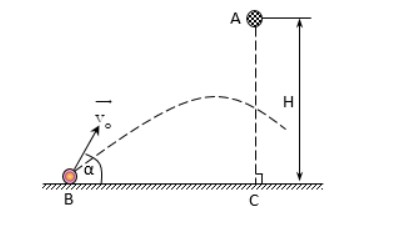
\includegraphics[scale=1]{../figs/VN10-2021-PH-TP014-1.jpg}
		\end{center} 
	}
	
	\hideall
	{	
		
		Phương trình vật thả rơi (vật I):
		
		$$x_1 = 0; y_1 = H -\text{0,5}gt^2.$$
		
		Phương trình vật II:
		
		$$\begin{cases}
			x_2 = L  - (v_0 \cos \alpha)t = H - (v_0\cos \alpha)t.\\
			y_2 = (v_0\sin \alpha) t - \text{0,5}gt^2.
		\end{cases}$$
	
		Để hai vật gặp nhau $x_1 = x_2$ và $y_1 = y_2$
		
		$$\begin{cases}
			(v_0\cos \alpha) t = H.\\
			(v_0 \sin \alpha)t = H.
		\end{cases} \Rightarrow \tan \alpha = 1 \Rightarrow \alpha = 45^\circ \Rightarrow v_0 = \sqrt{\dfrac{2Hg}{\sin 2\alpha}} = \SI{6}{m/s}.$$
	}
	\item \mkstar{2}
	
	
	{Vật được ném xiên góc $60^\circ$ với vận tốc $\SI{30}{m/s}$, lấy $g=\SI{10}{m/s}^2$, tính tầm xa và độ cao cực đại vật đạt được.
	}
	
	\hideall
	{	
		Tầm xa của vật
		
		$$L = \dfrac{v^2_0 \sin 2\alpha}{g} = \SI{77,94}{m}.$$
		
		Độ cao cực đại
		
		$$H = \dfrac{v^2_0\sin^2 2\alpha}{2g} = \SI{33,75}{m}.$$
	
	}
		\item \mkstar{2}
	
		
		
		{Ném xiên góc $45^\circ$ một vật với vận tốc $\SI{25}{m/s}$. Lấy $g=\SI{10}{m/s}^2$, tính vận tốc của vật sau khi ném $\SI{1,2}{s}$.
		}
		
		\hideall
		{	
			Ta có:
			
			$$\begin{cases}
				v_\text{x} = v_0 \cos \alpha = \SI{17,677}{m/s}.\\
				v_\text{y} = v_0 \sin \alpha - gt = \SI{5,677}{m/s}.
			\end{cases}$$
		
			Vận tốc của vật
			
			$$v = \sqrt{v^2_\text{x} + v^2_\text{y}} = \SI{18,6}{m/s}.$$
			
		}
			\item \mkstar{4}
		
		
		
		{Từ mặt đất một vật được ném xiên lệch với phương ngang một góc $\alpha = 45^\circ$ với vận tốc ban đầu là $\SI{20}{m/s}$. Lấy $g=\SI{10}{m/s}^2$. Viết phương trình chuyển động của vật và độ cao mà vật có thể lên tới.
		}
		
		\hideall
		{	
			
			\begin{center}
				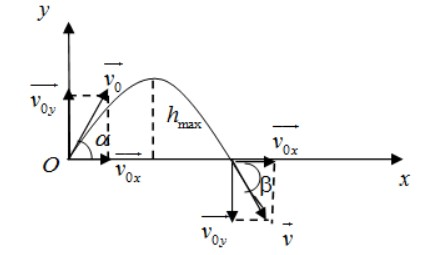
\includegraphics[scale=1.2]{../figs/VN10-2021-PH-TP014-2.jpg}
			\end{center}
			
		Thời điểm ban đầu
		
		Chiếu lên trục Ox có $x_0 = 0$
		
		$$v_{0\text{x}} = v_0 \cos \alpha = \xsi{10\sqrt 2}{m/s}.$$
		
		Chiếu lên trục Oy có $y_0 = 0$
		
		$$v_{0\text{y}} = v_0 \sin \alpha = \xsi{10\sqrt 2}{m/s}.$$	
		
		Xét tại thời điểm $t$ có
		
		$$a_\text{x} = 0; a_\text{y} = -g.$$
		
		Chiếu lên trục Ox ta có:
		
		$$v_\text{x} = \xsi{10\sqrt 2}{m/s}; x = 10\sqrt 2 t.$$
		
		Chiếu lên trục Oy ta có:
		
		$$v_\text{y} = 10\sqrt 2 - 10t; y = 10\sqrt 2 t - 5t^2.$$
		
		$$\Rightarrow y = x - \dfrac{x^2}{40}.$$
		
		Vậy quỹ đạo của vật là một parabol.
		
		Khi lên đến độ cao cực đại thì
		
		$$v_\text{y} = 0 \Rightarrow 10\sqrt 2 - 10t =0 \Rightarrow t = \xsi{\sqrt 2}{s}$$
		
		$$\Rightarrow h_\text{max} = y = \SI{10}{m}.$$
		}

\end{enumerate}